\documentclass[12pt, letterpaper]{article}

%==============Packages & Commands=================
\usepackage[utf8]{inputenc}
\usepackage{graphicx} % Graphics
\usepackage{indentfirst} % Tells LaTeX to indent every paragraph 
\usepackage{setspace} % To set line spacing
%\usepackage[longnamesfirst]{natbib} % For references
\usepackage{booktabs} % For tables
\usepackage{rotating} % For sideways tables/figures
\usepackage{amsmath} % Some math symbols
\usepackage[margin = 1in]{geometry}
\usepackage{subcaption}
\usepackage{mdwlist}
\usepackage{pifont}
\usepackage{array}
\usepackage{makecell}
\usepackage[normalem]{ulem}
\usepackage{colortbl}
\usepackage{url}
\usepackage{verbatim}
\usepackage{textcomp}
%\urlstyle{same}
\usepackage{appendix}
\usepackage{multirow}
\usepackage{dcolumn}
\usepackage{threeparttable}
%\usepackage[nolists]{endfloat} % Figures and tables at the end
%\usepackage{kotex}

%These allow for references to subfigures


%\newcommand{\R}{\texttt{R}\space} % Write R in typewriter font
%newcommand{\trans}[1]{{#1}^{\ensuremath{\mathsf{T}}}} % Transpose symbol 
%\captionsetup[subfloat]{position = top, font = normalsize} % For sub-figure captions
%\graphicspath{{Figures/}}
\DeclareGraphicsExtensions{.pdf, .png, .jpg, .tif, .tiff, .jpeg}

%\DeclareDelayedFloatFlavor{sidewaystable}{table} %Allows endfloat to handle sidewaystable
%\DeclareDelayedFloatFlavor{sidewaysfigure}{figure} %Allows endfloat to handle sidewaysfigure

%These packages for inserting blue hyperlinks in text (and for linking in-text references to references section)
\usepackage[bookmarks]{hyperref} %bookmarks option enables pdf bookmarks to be automatically generated
\usepackage[usenames,dvipsnames,svgnames,table]{xcolor}

\usepackage{authblk}

\usepackage{float}
\usepackage[multiple]{footmisc}
\usepackage{multirow,array}
\makeatletter
\usepackage{longtable}
\usepackage{cleveref}

\usepackage[authordate,backend=biber]{biblatex-chicago}

\addbibresource{references.bib}

\title{Taxes in the Time of Revolution: An Experimental Test of the Rentier State during Algeria's Hirak\thanks{We thank Michael Ross, Benjamin Graham, David Waldner, Giuliana Pardelli, Aaron Kaufman, Joan Barcelo and participants in the New York University Abu Dhabi political science seminar for helpful comments on this draft.}}
\author{Robert Kubinec and Helen V. Milner}
\title{Taxes in the Time of Revolution: An Experimental Test of the Rentier State during Algeria's Hirak}
\date{May 10, 2023}



\begin{document}



\maketitle

\begin{abstract}

We examine the rentier thesis that a government's control over oil resources should help it resist pressures for democratization. Our online survey experiment,  implemented during a nation-wide mobilization for regime change in Algeria known as the Hirak, used interactive experimental treatments to provide information about the Algerian government's subsidies for fuel resources and low value-added taxes. Based on a sample of 9,721 Algerians, we find that when Algerians learn about their country's relatively high level of fuel subsidies and low level of taxes, their assessments of the government's performance improves. However, we find null effects for outcomes involving demands for representation such as intentions to join protest movements. An analysis of treatment heterogeneity in terms of wealth shows that the wealthy became much more supportive of the regime in response to the treatment while in some cases the poor became much less so. This treatment heterogeneity appears to be related to divergent views among the wealthy and the poor concerning the goals of the protest movement, with the wealthy favoring institutional reforms while the poor prioritized redistributive justice.
    
\end{abstract}

\newpage

\doublespacing

The rentier theory, one of the longest standing conjectures of the determinants of regime type in comparative political science, argues that a state's control over natural resources is likely to promote a more authoritarian form of government \parencite{ross_does_2001,herb_no_2005,beblawi_rentier_1987}. The theory, which originated in the analysis of oil-rich states in the Middle East \parencite{crystal_oil_1990,beblawi_rentier_1987,ayubi_over-stating_1995}, has been shown to be a compelling factor in supporting authoritarianism through a wealth of cross-national studies, showing a robust association between the level of oil wealth and dictatorship, particularly since the 1970s \parencite{ross_what_2015}. In this paper, we experimentally test one of the core components of the rentier state theory: to what extent citizens limit their demands for representative government in response to changes in increases in receipts of oil-funded benefits from their non-democratic government \parencite{paler_keeping_2013,de_la_cuesta_oil_2019}.

This theory involves the taxation-representation trade-off \parencite{levi_rule_1989,tilly_coercion_1992, prichard_taxation_2015}. A state's control over oil resources provides it with a source of revenue which does not require regular tax collection or compliance, reducing citizen leverage in bargaining with the ruler over control of the resources. Our intention is not to test whether oil rents and taxes are actually substitutes--we assume  that they are --but rather whether the alleged reduction in taxes due to increased oil revenues empirically reduces demands for representative, and ultimately democratic, government.

Testing whether this trade-off between oil rents and democratic aspirations exists is difficult because episodes of regime change are  rare. To provide useful data, we examined a recent wave of popular mobilization in Algeria during 2019 known as the Hirak. This national protest movement endured for months up until the outbreak of the COVID-19 pandemic in 2020, and successfully forced the long-standing president, Abdelaziz Bouteflika, out of office. We fielded an online survey for several months during the early period of the protest movement from April to July 2019, recruiting a diverse sample of 9,721 Algerians. In our survey we embedded an interactive experiment which asked respondents for the amount they had spent on fuel subsidies and on goods covered by the value-added tax (VAT). To provide a plausible counterfactual per the rentier theory of an oil-free Algeria, we then showed them the increased amount they would spend on these items if they lived in Tunisia, a neighboring country which recently transitioned to democracy and does not have extensive fuel resources or subsidies. We supplemented these individualized treatments with a general informational message showing that the Algerian state's reliance on oil revenues has increased in recent years.

Our results show that the treatments improved respondents' perceptions of the government's performance, measured as its ability to combat corruption, provide public goods, implement reforms and guard stability. However, when we examine outcomes involving demands for accountability like intentions to protest, we find no clear differences between treatment and control groups, suggesting that the rentier state's resources are not able to affect these crucially important variables. When we examine treatment heterogeneity in terms of wealth, which was a core part of the interactive treatment, we find that wealthier respondents were much less likely to report a desire to join the protest movement upon receiving the treatment, while the opposite held for poorer respondents. Furthermore, the overall positive effects of the treatment on attitudes toward government performance are likewise concentrated among wealthier respondents. 

For these reasons, we believe that our results show that declining support for the rentier state among the wealthy is particularly problematic for rentier regimes. However, as we show with our survey data, the wealthy who supported the protest movement believed the movement would result in institutional changes but not changes to the level of redistribution. The effectiveness of our treatment among the wealthy in terms of dampening support for regime change suggests that these groups were prone to rethink their support for the Hirak once they realized the potential implications of revolutionary change on domestic political economy.

\section*{Background}

The rentier state is a theory that has profoundly influenced political science research since \textcite{mahdavy_hossein_patterns_1970},  \textcite{beblawi_rentier_1987}, \textcite{karl_paradox_1997} and \textcite{anderson_state_1987} explored the effects of oil resources on the nature of political institutions in the Middle East and Latin America. Since that time, a growing literature has documented strong associations between the presence of oil resources and more authoritarian forms of government \parencite{ross_does_2001,ross_oil_2012,ross_what_2015, andersen_big_2014}. However, it is difficult to narrow down the full range of theories to a precise set of causal factors \parencite{smith_rethinking_2021}. Scholarship has shown that the effect of oil on regime type may be conditional on a range of variables, such as the timing of regime change \parencite{houle_two-step_2018}, the degree of industrialization \parencite{brooks_oil_2016}, and the presence of income inequality \parencite{dunning_crude_2008}. 

While we acknowledge the many strands of the theory, in this article we focus primarily on the contention that oil revenues may reduce demand for representation by lessening citizens' tax burden in exchange for public and private goods. This can be understood as the demand side of rentier theory: to what extent rentier policies prevent contention from happening by reducing representative demands. There are other core components of the rentier thesis that can be understood as supply-side issues of state power, such as oil increasing a state's repressive capacity \parencite{ross_does_2001,bellin_robustness_2004,brownlee_arab_2015}, which can prevent regime change from occurring even if the majority of the population favors it. Our theoretical test primarily applies to the demand side rather than the supply side articulation given that our treatment affects individuals directly rather than by first changing institutions. For that reason our research is relevant to broader questions of governance involving bargaining with citizens for government revenue in exchange for public goods \parencite{bates_note_1985}.

\subsection*{Demand-side Theories of the Rentier State}

In general, the taxation-representation trade-off can be seen as a necessary, but not sufficient, condition for democratization. Early modern European states' demands for revenue and consequent increases in taxation are strongly linked to both increases in state infrastructural power and demands for more representation in the government \parencite{weiss_states_1995, dincecco_fiscal_2009, levi_rule_1989, bates_note_1985}. Recent studies show that this historical pattern also tends to hold among contemporary states as states that collect fewer taxes are also less democratic \parencite{slater_economic_2014}. This feature of contemporary state development may be explained by the widespread availability of sovereign finance that encouraged state expansion without the need for growing the tax base \parencite{migdal_strong_1988,queralt_war_2019}. As such, the taxation mechanism remains one of the best explanations for how a state's reliance on oil revenues could lead to more authoritarian government by reducing citizen claims on the state \parencite{jones_bedouins_2017}. If a state does not require citizens to contribute to its coffers, while still maintaining an acceptable level of public goods, then it may prevent redistributive conflicts because the cost of collective action to oppose the state is far greater than the benefits of the status quo.

It is perhaps unsurpising as a result that rentier state theory has its critics who allege that the theory is based on flawed cross-sectional comparisons \parencite{waldner_against_2015,herb_no_2005}. The theory seems to best explain resource-dependent countries in the Middle East, which also happens to be the most authoritarian region in the world \parencite{jamal_democracy_2008}. Despite the durability of authoritarian regimes in the region, it does not necessarily follow that authoritarianism is caused by states' discovery of oil resources. Rather, there could be early factors in state development which predisposed Arab governments to form more authoritarian governments. The subsequent exploration of oil resources may have served to lengthen a given leader's tenure but may not have affected the leader's propensity to use authoritarian means to retain power, as plausibly occurred in the Arabian Gulf in the first half of the 20th century \parencite{waldner_survivorship_2021}. Even if oil resources tend to reduce citizen claims on the state, survey evidence shows that Gulf citizens are prone to unhappiness with the rentier state if it is seen as corrupt or inegalitarian \parencite{mitchell_what_2019}.

%The main challenge in adjudicating these rival positions is the fact that we are studying a variable which we can almost never experimentally manipulate: oil resources. For example, to understand with  confidence whether oil resources are the main prop behind the Saudi Arabia's long-lived monarchical regime, it would be necessary to observe a Saudi Arabia both with and without oil resources. Comparing Saudi Arabia to other wealthy authoritarian nations such as Singapore is a limited form of inference as it is hard to find an appropriate comparison country. Furthermore, cross-sectional comparisons can obscure important anomalies, such as Kuwait, a country with ample oil resources yet also the longest-lived parliament in the Arab world \parencite{crystal_oil_1990,gandhi_political_2008}. Exploiting within-country variation in oil resources can at least partially alleviate these concerns \parencite{ross_what_2015}, but because oil resources are not exogenous to political development \parencite{waldner_survivorship_2021}, it is difficult to make fully identified causal inferences from panel data  alone.

%Problematically, employing country-year observations to test demand-side rentier theory introduces an ecological inference problem \parencite{king_solution_1997}. Aggregate measures of oil resources and outcomes such as levels of democracy obscure heterogeneity in individuals' responses to the rentier state. 

Our main theoretical contribution in this paper is to explore the conditional preferences that class groups have toward the rentier state. Existing theory tends to view citizen preferences as largely derived from the level of benefits they receive, but during times of contention, the definition of what constitutes largesse is the issue that citizens must decide. Furthermore, even if the level of benefits provided is large in absolute terms, unhappy citizens may still be upset based on comparisons they rely on to determine whether their share of the pie is reasonable. As we will show in this paper, people with varying wealth endowments are likely to judge the performance of the rentier state differently, and these endowments may also shape their willingness to engage in costly collective action.

%What is important to note is that this theory implicitly makes statements about the distribution of preferences among the population. If citizens receive benefits from the state without representation, then they should reduce their demands for representation. However, until recently, much of the work about demand-side rentier state theory made use of country comparisons, which necessarily obscure questions about how individuals respond to the largesse of the rentier state. 

While limited to date, experimental approaches have shed light on the taxation-representation trade-off at the micro level. \textcite{paler_keeping_2013} provided initial support for the trade-off by showing that citizens in resource-rich areas expressed greater demands for accountability following the discovery of resources. Quasi-experimentally, \textcite{gadenne_tax_2017} showed that Brazilian municipalities were more likely to invest increases in revenues from taxes in public goods like education, but not so with ``unearned" revenues like grants, which the municipalities used for discretionary projects. \textcite{de_la_cuesta_oil_2019} finds that accountability demands by citizens depend on citizens' perceptions of ownership over the revenue, not just its source. In other words, citizens of rentier states do not blithely ignore the government, but rather conditionally support the regime if it is seen as meeting its implicit contract to share the wealth \parencite[67]{ross_oil_2012}. 

%We know little, for example, about how wealthier or poorer people may differentially respond to shortcomings in the rentier state, though we do know that inequality writ large could play an important mediating factor \parencite{dunning_crude_2008}.

We build on this experimental literature by examining a context in which regime change is a serious issue of contention. For these reasons, we would expect that theories of regime change in political science and economics would be relevant \parencite{acemoglu_economic_2006,boix_democracy_2003,acemoglu_persistence_2008}. We can understand the rentier state as an attempt to appease salient class groups and avoid regime change. In terms of threats from below \parencite{przeworski_conquered_2009}, if inequality increases and the rich are able to capture the lion's share of the rentier state's public goods, then the willingness of the poor to engage in costly mobilization to oppose the regime also rises. Similarly, as \textcite{dunning_crude_2008} shows, the rentier state can help mitigate private sector inequality, but only if public goods represent true redistribution to the poor. For these reasons, to avoid popular mobilization, rulers should try to make the rentier state as inclusive as possible, which Algeria was able to do during the earlier Arab Spring protest movement in 2011 by dispensing subsidies targeted at consumers. 

However, rulers also need to keep elites co-opted, who often represent a more immediate threat in terms of regime survival \parencite{gehlbach_investment_2011,marinov_coups_2014,ansell_inequality_2014}.  In fact, \textcite{geddes_autocratic_2014} show that oil has its greatest effect on authoritarian durability by avoiding coups from rival factions. Popular mobilization, by contrast, is relatively rare and can also be contained with repression \parencite{bellin_robustness_2004}. As a result, regimes need to appease the wealthy who often hold greater political staying power than the poor \parencite{waterbury_egypt_1983,waldner_state_1999,haber_politics_2003}. Prior research shows that the wave of protests that swept across the Arab world during 2011 was closely related to disenchantment among wealthier Arabs toward the decaying performance of the public sector \parencite{diwan_understanding_2013}. 

Fully testing dynamic models of regime change is beyond the scope of this paper, but by employing a research design with granular treatments that vary by individuals in terms of wealth, we can probe the social and class cleavages that affect regime strategies and the responses of different groups to problems in the regime \parencite{magaloni_voting_2006, de_la_o_conditional_2013,haggard_inequality_2012}. For the poor, rentier benefits may have a very different effect on their political attitudes and behavior compared to the rich, which likely depends on the coalitional basis of the rentier state in question \parencite{waldner_state_1999}. These potentially divergent theoretical predictions provide us an opportunity to better understand how the taxation-representation tradeoff matters in the midst of a highly salient episode of regime instability.

%What is important to the taxation-representation trade-off is the counterfactual: what would citizens demand if the regime did not have access to oil resources? If the theory holds, then reduced oil revenue should lead to increased taxation and subsequent demands for representation. It is this central principle that we seek to test experimentally by examining demands for the strongest form of accountability: regime change. By directly incorporating individual heterogeneity in terms of wealth into the treatment, we can further disaggregate the treatment's effects by possibly quite salient class divisions. 

%Additionally, we are interested in the conditional effects of the rentier state in terms of inequality. It seems to follow logically that a person's position in the wealth distribution would affect how they perceive government largesse \parencite{mitchell_what_2019}. The poorest may not spend as much on goods covered by taxes or earn enough income for tax benefits to become appreciably large. By comparison, if the rentier state focused more on pro-poor policies like conditional cash transfers and subsidized housing, they might be able to affect the views of the poor to a higher degree \parencite{magaloni_political_2010,de_la_o_conditional_2013}. In fact, if the poor perceive the rich as obtaining more of the benefits of the rentier state due to increasing inequality \parencite{haggard_inequality_2012}, then there is reason to believe that the rentier state could help create grievances rather than suppress them. For these reasons, in addition to the overall effect of the rentier state on actions and attitudes towards democracy, we also want to know whether its effects are conditional on factors we have reason to believe should matter for the comparative value of benefits obtained from the state.

\subsection*{Algeria During the Hirak}

We focus our study on Algeria as an excellent case for examining the taxation-representation trade-off proposed by rentier theory because, over the last twenty years, the regime has had to face challenges to its patronage and welfare benefits due to population growth. Most recently, Algeria's Hirak protest movement in 2019 provided an ideal context in which to investigate the efficacy of the rentier state as it represented a rare episode of mass contention in a state with significant oil resources. While Algeria's petroleum resources never reached a per capita level of the small Gulf states, it possesses a considerable share of the world's oil resources--12.2 billion barrels of proven reserves--and for decades was able to sustain a quality of life above the regional average for its citizens. In addition to its natural resource endowments, Algeria is distinctive for its long-lived authoritarian regime.

Algeria has had authoritarian government since its hard-fought independence from France in 1962. Starting with the revolutionary leader Ahmed Ben Bella in the 1960s, Algeria experienced a series of dictators who relied on the unquestioned dominance of the armed forces to maintain control. The security state further survived a decade-long war with the Islamic Salvation Front following botched elections in 1992, ending with the election of Abdelaziz Bouteflika to the presidency in 1999. Though Bouteflika did not have a military career, he was elected with the military's support, and he preserved the military's prerogatives over budgeting and lucrative economic enterprises \parencite{dillman_state_2000}. On the whole, after the conclusion of the civil war of the 1990s, Algeria remained quite stable during Bouteflika's rule  until the outbreak of the Hirak protests. 

While it would be unrealistic to chalk up the regime's longevity solely due to oil, the presence of a high level of natural resources appeared to paper over the diminished legitimacy of the regime as the war for independence became a distant memory. One of the best examples of the regime's employment of rent to counter instability occurred during the Arab Spring, which started in neighboring Tunisia in late 2010. Although protests did spread from Tunisia to Algeria in the spring of 2011, an increase in government spending on food subsidies appeared to keep the protests from spiraling out of control.\footnote{See \url{https://www.iemed.org/publication/the-arab-spring-is-algeria-the-exception/}.} Bouteflika further announced liberalization measures, which while partial and ultimately lacking implementation, increased benefits for Algeria's citizens.\footnote{See \url{https://www.iemed.org/publication/the-arab-spring-is-algeria-the-exception/}} 

While analysts acknowledge this largesse as contributing to the regime's stability, it was also clear that the rentier state might not always deliver. As Lahcen Achy wrote in 2012, ``if the price of oil suddenly drops, reducing the government’s ability to control the budget deficit, this could fuel popular anger... to me, it is only a matter of time." Similarly, Yahia Zoubir opined in 2016 that ``strikes, protests and riots are routine," although ``the regime has been able to address them through payoffs in the form of higher salaries or housing vouchers." \nocite{zoubir_algeria_2019,achy_algeria_2012}

\begin{figure}
    \centering
        \caption{Algerian Fiscal Capacity and Oil Rents}
    \label{fig:algrev}
    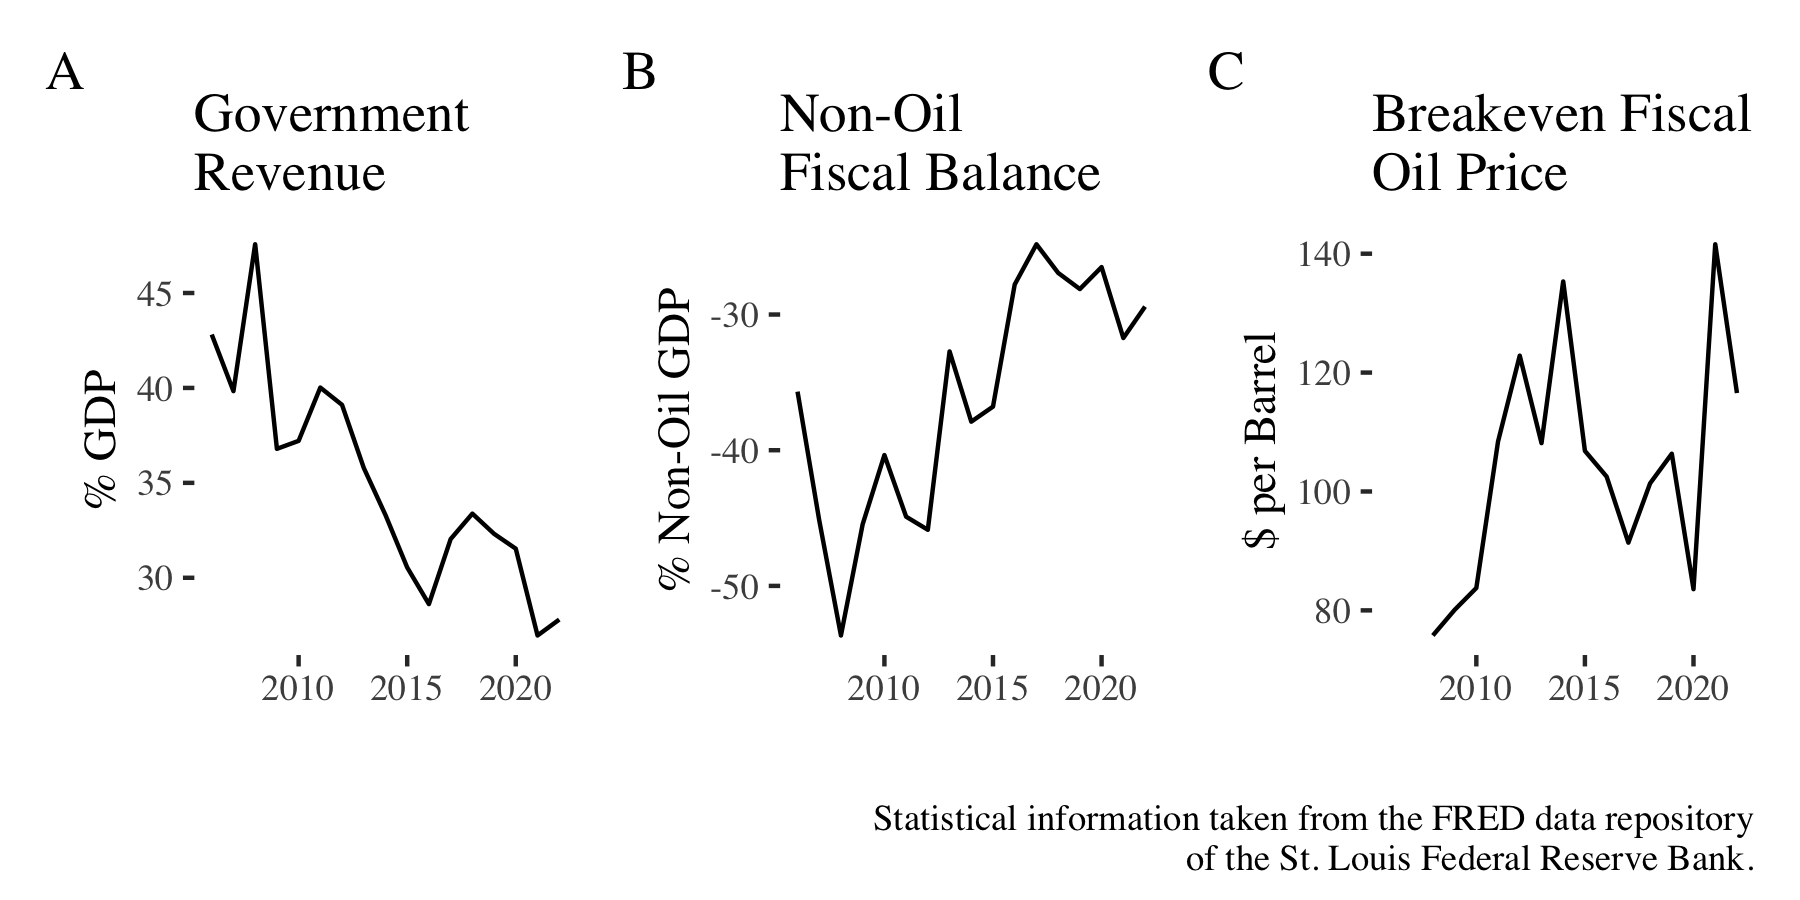
\includegraphics[width=\linewidth]{plots/oil_fiscal_capacity.png}
\end{figure}

The regime's problems came from the fact that, although its natural resource revenues remained quite large, they did not increase in tandem with Algeria's population, creating stress on patronage policies and public good provision. Algeria, like many other Arab states, used state-led development to create a new middle class that depended on a stable supply of government jobs as a path to advancement \parencite{diwan_understanding_2013}. The macroeconomic data for Algeria shown in Figure \ref{fig:algrev} reveals the declining coverage of government expenses with oil receipts. Between 2010 and 2020, government expenditure as a percent of GDP in panel A in Figure \ref{fig:algrev} declined from the high 40s to the low 30s. At the same time, the fiscal balance of the government in terms of non-oil GDP (panel B), which is a measure of the extent to which the government relies on oil revenues, declined from -50\% to about -30\%. The reason for these declines had to do with the needs of a growing population and largely flat oil production at around 500,000 bpd. Consequently, the breakeven oil price in panel C, or the price at which the government can adequately fund its budget, grew from under \$80/barrel at the start of the decade to more than \$120/barrel by the end, which left the government in an unsustainable fiscal position. 

As such, while the system proved remarkably durable during the Arab Spring, informed observers had noted cracks in the rentier system.  However, these conditions existed for some years before an aging Bouteflika, troubled with poor health, nonetheless decided to push for a fifth term as president. Algerian activists seized the moment, and on February 22, 2019,``millions of Algerians" participated in a march demanding Bouteflika's resignation.\footnote{See \url{https://www.hrw.org/news/2022/02/21/algeria-3-years-repression-protest-tightens}} While survey data is limited, up to 50 percent of Algerians may have shown interest in turning out to protest during the movement's high point in the spring and summer of 2019 \parencite{grewal_algerias_2019}. Remarkably, this high level of participation continued for months as Algerians turned out each Friday, making use of focal points to sustain momentum \parencite{ketchley_trends_2020}. While the protests decreased in size, the weekly activism only ended when COVID-19 cases appeared in Algeria and the government mandated an end to gatherings.\footnote{See \url{https://www.arab-reform.net/publication/the-future-of-the-algerian-hirak-following-the-covid-19-pandemic/}} 

The Hirak's main achievement came from forcing Bouteflika to step aside, one of its original demands. However, the movement was unable to stop the election of another regime insider, Abdelmadjid Tebboune, to the presidency in December of 2019.\footnote{See \url{https://www.hrw.org/news/2022/02/21/algeria-3-years-repression-protest-tightens}} Because of these limited successes, it is important to note that state spending on salaries and welfare measures was not the only way that oil wealth influenced the success of the protest movement. Algeria's military is also much larger than its neighbors and oil rents helped fund their security apparatus that targeted protest leaders \parencite[52-55]{brownlee_arab_2015}. While Bouteflika's resignation signaled an important victory for the protesters, it is clear that the movement did not ultimately succeed in regime change \parencite{grewal_why_2021}. 

For this reason, the ``pouvoir'', or system of elites, that many activists sought to destroy remains intact as of the spring of 2023. Even though Algeria's oil largesse provided housing, jobs and education, it is still true that the military and affiliated political elites captured the lion's share of the rentier system's benefits \parencite{dillman_state_2000}. While Algeria's revolution replaced the French occupiers, over time it created a new, domestic elite who had no qualms about ensuring their continued access to valuable rents. As such, Algeria is no exception to the patterns of crony capitalism and corruption prevalent in the region \parencite{malik_introduction_2020}. Replacing the leader without affecting the system that reproduced these inequalities could not result in lasting change, as the protest organizers knew well.

Concerns over elite bias in institutions figured prominently in the protest movement, suggesting that wealth endowments may have affected how people perceived the relative importance of the rentier state. Survey data from the  Arab Barometer in 2019 found a plurality of respondents (41\%) cited corruption and the quality of public services as the most important issues facing the country \parencite[4]{robbins_algeria_2019}.  Unsurprisingly, the government's response to the Hirak was to appear as though it was rooting out corruption, indicting prominent regime figures and businesspeople on abuse of power and unjust enrichment \parencite{marwane_after_2021}. As a result, we have prior reason to believe that not only the quality of the rentier state was at issue, but also whether benefits were being equitably distributed across class divides in the country.

To summarize, during an episode of regime contention like the Hirak it is clear that there were a significant number of people who were upset with the regime's policies and, by extension, with the performance and legitimacy of the rentier state. Given the salience of the issue, it would seem to be an appropriate time to ascertain to what extent the rentier nature of Algerian institutions helps depress protests. By the presence of protests we might infer that the rentier state's depressive effect on grievances is weaker than it was before, and the very real nature of regime contention also suggests that the rentier state's future is far from certain. For this reason, there should be a substantial number of people who, on the margin, might change their perspectives about the performance and legitimacy of the regime given new information.

\section*{Research Design}

Our research design aims to experimentally test the taxation-representation part of rentier theory using individual level data in a country that had a plausible chance of undergoing a regime transition. While we cannot manipulate Algerian institutions or oil deposits, we can influence the available information respondents have about the generosity of their rentier state in regional comparison. We pre-registered two hypotheses prior to our study, which we list below:

\begin{quotation}
H1: A higher level of gasoline subsidies relative to neighboring democratic countries will encourage pro-regime attitudes and actions among citizens in a dictatorship.
\end{quotation}

\begin{quotation}
H2: A lighter tax burden relative to neighboring democratic countries will encourage pro-regime attitudes and actions among citizens in a dictatorship.
\end{quotation}

As with any manipulation, we need to be aware of what the range of plausible counterfactuals is. It would seem impractical to try to compare Algeria to a counterfactual Algeria without oil or a counterfactual Algeria with democracy. Presumably so many other institutional and political variables would also change such that posing such a comparison to Algerians would result in unintelligible answers.

Instead, we compare Algeria to its immediate neighbor, Tunisia. Tunisia is a natural reference point because it has a long shared history with its neighbor, including decades spent under French colonization and similarly authoritarian institutions in the post-colonial period. However, Tunisia is different from Algeria in two crucial aspects: first, Tunisia transitioned to democracy in 2010 during the heady days of the Arab Spring.\footnote{We note that the anti-democratic actions of President Kais Saied since 2021 have put the viability of the country's democratic institutions in doubt. However, President Saied was not elected into office until after this study was completed.} Second, Tunisia has never had access to the vast natural resources of its neighbor. We think that Algerians were quite likely to rely on comparisons to neighboring countries during their period of regime contention due to the well-known heuristics of availability bias \parencite{weyland_arab_2012}. 

In fact, it is quite plausible that if Algeria did not have access to oil-funded patronage in 2010, it might have transitioned to democracy as Tunisia did in 2011. As such, this counterfactual comparison is based on a potential path that Algeria could have explored in recent history. \textcite{benstead_why_2014} reports that Tunisia's struggles in the post-transition period influenced Algerians' perceptions of the strengths and weaknesses of democracy as a form of government, suggesting that Tunisia is the most relevant empirical model for Algerians when it comes to potential regime change. In fact, \textcite{ross_oil_2012} uses Tunisia and Algeria to demonstrate how differences in oil endowments shape their remarkably different sizes of government despite the countries' similarities (pp. 29-30). 

As such, we  use Tunisia as a empirically-grounded counterfactual for the taxation and representation trade-off: Tunisia has a much more representative and accountable government, but also a much higher tax burden for a similar level of social services. Tunisia can serve as a baseline for Algerians to evaluate the generosity of the benefits they obtain in exchange for continued authoritarianism. In other words, if Algeria did not have both oil \emph{and} a ruler willing to share the wealth to an acceptable degree, it might look like Tunisia, a more democratic state with a higher tax burden. 

Of course, this comparison is only relevant to the extent that the theory itself holds. For example, it is quite plausible that Tunisia's transition to democracy and Algeria's authoritarianism had little to do with the former's lack of resources and the latter's abundance. If such a trade-off does not exist, then there is nothing stopping Algerians from deciding that they would prefer to receive their oil wealth under democracy regardless of the current regime type. However, if the trade-off does not exist, then informing Algerians about the nature of Tunisian public goods should result in null treatment effects and falsification of the rentier thesis that oil endowments diminish demands for representative government. If the rentier thesis does influence demands for democratization, then comparisons between oil-rich authoritarian countries and resource-poor democratic countries are a logical implication of the theory. 

%In a sense, this experiment is directly testing the implied counterfactuals of the panel data observational studies underpinning the  resource curse literature.

%Of course, we could also have tried to compare Algeria with other resource-rich countries so long as the regime type in these countries differs, such as regimes that are authoritarian but more stable or regimes that are more democratic yet have extensive natural resources.  While this comparison in principle is relevant--these counterfactuals approximate other ways that a country's institutions or resources could change vis-a-vis rentier theory--practically speaking it is more difficult to compare Algeria to such a country given the relatively low salience and greater heterogeneity of plausible candidates, such as Saudi Arabia or Norway. 

To make this comparison concrete, we designed two experimental comparative treatments based on three distinct policy regimes: gasoline subsidies, taxi rates, and value-added taxes (VAT). As a petro state, Algeria passes on some of its hydrocarbon revenues to citizens by subsidizing gasoline, resulting in a divergence in gasoline prices between Algeria and Tunisia.\footnote{In fact, gasoline smuggling is a lucrative occupation for residents of the mountainous Algerian-Tunisian border \parencite{ghanem_algerias_2020}.} Although the government does not score very highly on budget transparency, analysts were able to estimate the value of fuel subsidies at \$20b USD in 2014. While the Algerian government subsidizes other goods, the sheer value of these subsidies, and their close connection to the value of domestic hydrocarbon production, makes them an important part of any experimental treatment related to the rentier state and bargains over redistributive largesse.

In addition, gasoline subsidies have previously been shown to be inimical to democratization \parencite{fails_fuel_2019}, suggesting they are an important mechanism besides tax burdens through which rentier largesse affects political calculations. While fuel subsidies are inherently regressive, they are still quite popular because the poor benefit even if the rich benefit to a larger degree on average \parencite{kyle_local_2018}. In other words, even if the rich obtain more of the subsidies on average, it is unlikely that the poor will rise up to protest the fuel subsidies because oil-related expenses may still make up a significant share of their monthly expenses. 

We include taxi fares as an alternative to gasoline subsidies in order to extend this treatment to cover Algerians who did not own cars. The difference in gasoline prices between Algeria and Tunisia should also result in differences in taxi prices, which affect most of the population. For this reason, our gas treatment uses either retail gasoline prices or taxi fare prices depending on whether the respondent owned a car. To estimate gasoline prices, we use historical gas pump prices for both countries.\footnote{See \url{https://www.globalpetrolprices.com/Algeria/gasoline_prices/}.} Estimating taxi prices is somewhat more difficult, though we are able to use crowd-sourced websites to come up with plausible average rates of taxi fares for both countries.\footnote{See \url{https://www.numbeo.com/taxi-fare/country_result.jsp?country=Algeria}.} 

We acknowledge that using separate treatments means that each group will receive a different stimulus even if the aim is the same. In our main results we pool these treatments together, and in the appendix we report disaggregated treatments as well. We note that differences between these treatment groups cannot necessarily be attributed to differences in the treatments given that treatment assignment is endogenous to owning car and possibly other causal factors related to car ownership.

We chose to operationalize taxation in terms of indirect, value-added taxes because data on direct taxes, such as income taxation, is difficult to obtain and potentially of low quality, especially in Algeria. In addition, direct taxes represent only a small part of the taxation burden in much of the region \parencite{jewell_fair_2015}. For VAT rates, we can draw on helpful existing research of both nominal rates and total product coverage. Algeria's VAT rate of 19\% is nominally the same as Tunisia's. However, the Algerian VAT is applied to far fewer goods according to research on VAT coverage rates by the IMF.\footnote{See \url{https://www.imf.org/external/pubs/ft/sdn/2015/sdn1516.pdf}.} As such, the effective VAT burden is far lower in Algeria than in Tunisia.

We then use these observed prices and VAT coverage rates to determine how much an individual might spend on gasoline, taxis or the VAT in Tunisia given a similar amount spent in Algeria. Table \ref{calc} shows these calculations for a hypothetical amount of 100 DZD spent in Algeria. A respondent will receive the gas treatment if they reported owning a car and a taxi treatment if they did not. We report these two treatments as one combined treatment in the results.

\begin{table}[H]
\caption{Treatment Calculations}\label{calc} 
\begin{tabular}{@{}lcc@{}}
\toprule 
Type         & Amount Spent in Algeria       & Counterfactual Spent in Tunisia \\ \midrule
Gasoline     & 100 DZD                       & 200 DZD                         \\
Taxis        & 100 DZD                       & 117 DZD                         \\
Spent on VAT & 3 DZD (for 100 DZD in Goods) & 7 DZD                       \\ \bottomrule
\end{tabular}
\end{table}

As can be seen, hypothetical expenditures on both gas and goods covered by the VAT are roughly double what a person in Tunisia might pay relative to Algeria. Expenditures for taxis in Tunisia are not twice as high as in Algeria likely due to the fact that taxi rates are kept arbitrarily low in Tunisia, which has resulted in taxi driver protests in recent years.\footnote{For example, see \url{https://arabtradeunion.org/en/tunisia-a-strike-for-the-individual-taxi-drivers-on-the-5th-of-november?lang=2}.} In any case, it is clear that the rentier state in Algeria does permit less taxation and a higher rate of subsidy of petrol relative to the less well-endowed Tunisia. We believe that this information--at least in this precise a form--would be relatively novel for Algerians and would provide an informative baseline for them to evaluate the amount that they are benefiting from the rentier state and whether that trade-off might justify continued authoritarianism. 

The treatment text is as follows:

\begin{quotation}
Based on what you entered, you paid \emph{[respondent amount]} DZD for [gasoline/taxis/VAT goods] last year. If you lived in Tunisia, a democracy, where [gas/taxis/VAT] receives fewer subsidies, you would probably have spent \emph{[re-calculated respondent amount]} DZD on [gas/taxis/VAT].
\end{quotation}

The inclusion of the phrase, ``a democracy," was an attempt to ensure that respondents would make the correct inference as to why Tunisia was the baseline for them to comparison with. However, out of concern that this suggestion would be too subtle, we also added the following text to 50\% of the treatments:

\begin{quotation}
However, Tunisia also has free and fair elections where people can hold politicians accountable.
\end{quotation}

This additional line of text provided some additional internal validity at the risk of some heavy-handedness. This treatment-within-treatment will help us understand if respondents' perceptions of the treatment is influenced by more subtle or more direct phrasing.

While these treatments provided information specific to individuals about their exposure to the rentier state, we also employed a treatment which contained general information about Algeria's oil resources. This treatment exploits the same counterfactual as that of the panel regressions mentioned earlier: over-time change in the amount of fuel earnings. If Algeria's dependence on oil revenues increases, then taxation makes up a smaller share of overall government revenue. To capture this version of the treatment, we showed the following text to a subset of respondents:

\begin{quotation}
For every 100 DZD the Algerian government collected in 2016, 34 DZD came from oil and the rest (66 DZD) came from people's taxes. Since then, however, the government has become *more* reliant on oil for each 100 DZD it spends.  By last year oil as a share of the government's money accounted for 40 DZD for every 100 DZD collected.
\end{quotation}

By comparison to the individual level treatments, this treatment examines how Algerians might respond to information about the overall state of their oil resources. It is likely that this information is relatively novel for respondents as it involves specifics about how much the Algerian government currently relies on oil resources. Theoretically, we would expect this information to have similar kind of effect to the individual treatments because it is showing that the government is obtaining more revenue from oil resources as opposed to other sources such as taxes. 

We note that we are implementing these treatments in a very high salience environment--literally, a revolution in the making--in which government policies and legitimacy are hotly debated. As such, priming effects are unlikely to have much if any role in the interpretation of the treatment. Rather, the treatments' efficacy comes by offering new information that respondents would be very unlikely to have had pre-treatment. Given the high salience of the legitimacy of the rentier state, we can be quite confident that any effect of the treatment will come via this new information, not simply by prompting respondents to think about the government in general. If our aim was to identify the effect of primes, this level of background salience would be problematic, but as our aim is to identify the effect of new information about the respondents' benefits from the rentier state, it is an ideal context because we expect respondents to give the treatment's information serious thought as it relates to ongoing political discourse. 

To test the theory, we need to operationalize variables with survey questions that are the most relevant to the theory. Given that there are diverse strands of the theory, we also examine several different outcomes, including Algerians' attitudes towards their government and its provision of public goods, and also their willingness to take specific actions which could be interpreted as making representative demands in terms of regime change. We label the first set of outcomes as \emph{governance} measures, and the second as \emph{accountability} measures. The first set of measures covers a wide set of criteria for evaluating the quality of Algeria's government, but is only probabilistically correlated with potential demands for representation. In other words, a respondent could reduce their perception of the government's performance without necessarily increasing representative demands. At the same time, public goods are a key criteria underlying the bargains that rentier state theory supposes citizens make with the regime.

To address political action more directly, we also include measures which correspond to the respondent's support for and confidence in the current regime, including willingness to join protest and to keep liquid financial assets within the country. Because the Hirak had explicitly democratic goals such as for free and fair elections, we know that willingness to protest represents a relatively costly way of making demands for representation. Furthermore, we know that there is substantial variation in this DV given that protest intentions changed dramatically over the course of the Hirak \parencite{kilavuz_ghosts_2023}, which makes it more likely that we would be able to cause a change in protest intentions. While both sets of outcomes are relevant, our interpretation of rentier state theory suggests the accountability outcomes are more direct tests of the taxation-representation tradeoff, though we note that a consensus in the literature on this question does not exist as of yet.

\subsection*{Governance Measures}

Our governance measures come from the following survey question:

\begin{quotation}
How would you rate the government’s performance in these areas on a scale of 1 to 10:
\end{quotation}

\begin{tabular}{@{}ll@{}}
\toprule 
1 & Providing employment for its citizens \\
2 &Helping Algerians obtain health care and a quality education \\
3 &Ending corruption among government officials \\
4 &Reforming in response to citizens’ concerns \\
5 &Maintaining stability and social order \\ \bottomrule
\end{tabular}

\vspace{1cm}

\subsection*{Accountability Measures}

Our accountability measures come from the following survey question:

\begin{quotation}
On a scale of 1 being very unlikely and 10 most likely, are how likely are you to take the following actions in the next 3 months:
\end{quotation}

\begin{tabular}{@{}ll@{}}
\toprule 
1 & Participate in a street protest \\
2 & Visit a government official to complain about government services \\
3 & Move personal funds to bank accounts overseas \\
4. &Transfer funds from Algerian currency to other currencies \\ \bottomrule
\end{tabular}

It is important to note that our actions include those which can unambiguously represent demands for more representation, i.e. joining street protests with a movement calling for the overthrow of the regime, and others that are somewhat more ambiguous. Transferring funds into and out of Algerian currency or moving money overseas can be a way of holding the regime accountable by moving assets out of the country \parencite{bates_note_1985}. Using multiple measures allows us to track the effect of the treatment across diverse ways of understanding confidence in the regime, though joining protests would seem to be the most direct way of expressing opposition given the size and strength of the Hirak.

All of the outcomes and experimental treatments were pre-registered, although the additional treatment text mentioned above was added after the pre-registration was filed. While the pre-registration includes a power analysis, it does not include any description of additional analyses such as subgroup effects, mainly because of limitations of the speed with which the experiment had to be prepared and launched in the early days of the Hirak. For that reason, any such subgroup analyses should be considered exploratory, and we limit ourselves to examining treatment heterogeneity in the main text that is a part of the treatment, i.e., by examining respondents' wealth endowments. We include additional exploratory analyses of subgroup effects in the appendix. 

As we discuss in the next section, our actual data collection exceeded our pre-registered power projections by a significant margin, so we do not believe that examining additional treatment interactions will necessarily result in spurious inference as a result of ``the garden of forking paths" \parencite{gelman_garden_2013}. 

For these reasons, we consider our analysis of wealth endowments to be an appropriate analysis given the ample power to detect effects and the fact that the treatment is targeted based on respondent wealth.

\section*{Data}

Collecting survey responses in the midst of a national upheaval in a highly repressive authoritarian regime necessitates employing techniques that are more flexible than traditional face to face surveys. To do so, we recruited 9,721 Algerian residents (excluding members of the military and security forces) from April to July 2019 via advertisements on Facebook. Facebook is by far the most popular social medium in the Middle East, used widely across age demographics and by official authorities \parencite{dennis_media_2016}. Our advertisements, which asked for Algerians' opinions about the protests, attracted considerable attention, allowing us to recruit our nearly 10,000 respondent sample with a budget of only \$5,000, which included providing a 100 DZD mobile credit (approximately \$0.75) to all who finished the survey.\footnote{Not all respondents received a credit, either because they did not provide a mobile number or they did not provide a valid mobile number.} In total we have 2,439 respondents in control, 3,919 respondents who received at least one version of the fuel subsidies treatment (cars or taxis), 2,366 respondents who received the tax treatment, and 997 respondents who received the oil revenue message. The treatment groups are not equally-sized because the oil revenue message was added after the survey began to be fielded. The fuel subsidy treatment group is larger to allow for the two treatment types, cars or taxis, to be differentiated. 

We note that the size of these treatment groups permits highly precise inference on even very small treatment effects. Our actual sample size of 9,721 exceeded the upper bound of our projected pre-registered power analysis by nearly 5,000 respondents, permitting us to add an additional treatment arm. While false positive results are only one possible threat to inference, we believe that our experiment is powered enough to detect an effect if one exists and is of any appreciable size. Furthermore, the design is well-powered for examining sub-group and interaction effects, and as we discussed above, it is unlikely we could find large subgroup effects from sampling variation alone.

Although the online design was both cost-effective and possible to field in a limited time frame, it was also necessary due to Algeria's heavy-handed restrictions on social science research, which have allowed very few surveys over the past several decades. In addition, online designs have an advantage in terms of safeguarding respondents' privacy, who can take the survey in secure locations, as well as reducing risks for enumerators who do not need to be on the ground. Aside from the voluntary collection of mobile numbers for reimbursement, the survey was anonymous, permitting more confidence in the safe and valid collection of opinions about Algerian politics. Online surveys have been shown to be better at collecting sensitive information \parencite{chang_comparing_2010}, reducing our concern over sensitive survey bias. In addition, political opinions and protest participation were not particularly sensitive during this time period in Algeria thanks to the constant presence of public protesters making radical demands against the regime \parencite{kuran_sparks_1989}. 

%Finally, we note that all of the information we provided in the experiment is truthful so far as available data permits. Because this information could influence Algerians' political actions, it is important that it provide them with accurate baselines about which to make decisions. While this information may have led some to participate in the protest movement, we note that the size of our sample means that it was unlikely to affect the success of the movement, which numbered in the hundreds of thousands. Furthermore, while we recorded the respondents' intentions to protest, we did not explicitly advocate for or against any political side in the survey.

The sample did not conform exactly to Algeria's population demographics, as can be seen in Table \ref{desc}. The differences are most pronounced for age demographics, with over-representation in the under 30 groups and relatively few respondents over the age of 65. On the other hand, we matched census totals for the total number employed and also for sex.

To adjust for potential bias, we implemented multiple regression with post-stratification (MRP), a powerful method utilized heavily in online survey research \parencite{wang_forecasting_2014}. To do so we constructed a contingency table of the population totals of Algerians by district, age and gender, and re-weighted our model predictions by each of the 864 cells in the contingency table. Because MRP is a model-based method, the uncertainty from using point predictions for specific district-age-gender cells will propagate into our treatment effect estimates. For example, because we use MRP to predict values for all over-65 cells in the census data, we force our estimates to incorporate our uncertainty about this small proportion in our data relative to the population. For this reason, we believe that we can plausibly interpret our estimates as being nationally representative along these three dimensions. The large size of our sample further allows us to be more confident that this method will work well. For example, even though only 2.5\% of the sample is over the age of 55, this subgroup still totals 131 respondents, giving us reasonable statistical power for adjustment even for this older demographic.

\input{tables/descriptives}

While much of the data is straightforward to analyze given that it was collected via an online instrument, we did need to perform additional validation to create a measure of socio-economic resources (SES). To do so, we employed a latent variable model \parencite{kubinec_generalized_2019} and collapsed a wide range of indicators of both income and wealth. We did so because, as is often the case with survey data, considerable measurement error exists in any single indicator, including monthly  income. Furthermore, to understand how respondents may be affected by the rentier state, we need to know the respondents' overall level of resources rather than simply their current  monthly income. 

%Some respondents who were students, for example, may have very wealthy families and consequently a high standard of living even if their monthly income is zero. 

The inputs to our latent variable model included whether a respondent owned a car, a farm, a small, medium or large business; a house, whether they had a domestic or foreign bank account, sex, age, opinions about the state of the economy, level of education, a categorical measure of monthly income, the respondent's governorate, location (rural, urban or suburban), and also the amounts respondents reported spending on fuel, taxis and VAT goods in the experimental treatments. Combining all of these with appropriate statistical distributions and employing a two-stage correction for non-ignorable missing data \parencite{kubinec_generalized_2019}, we then estimated an SES scale which is shown in Figure \ref{ses}. Although the scale is continuous, it shows discrete breaks due to the fact that categorical variables with a strong effect on SES (ownership of homes or businesses) were included in estimation. The full list of discrimination parameters (i.e., factor scores) for all covariates in the SES scale is shown in Figure 2 in the appendix.

\begin{figure}
    \centering
    \includegraphics[width=0.9\linewidth]{plots/ses_hist.png}
    \caption{Histogram of SES Scale from Survey Data}
    \label{ses}
\end{figure}

It is important to note that the SES scale is a latent variable, and as such it does not need to follow a power law distribution like reported income. Rather, it is useful for making relative comparisons between respondents in terms of their wealth position rather than the absolute amount of income or they possess. We do note that relatively few of the respondents are either very poor or very rich (scores above or below +/- 5), with the majority reporting at least some income or other source of support. 

%In other words, while respondents were not wealthy on average, neither do we see absolute destitution. 

\section*{Results}

In the appendix we report the treatment interactions with the additional text incorporated about Tunisia's free and fair elections. These results do not show any noticeable increase or decrease in treatment effectiveness, suggesting that the simpler wording was able to communicate the nature of the trade-off we wanted respondents to make between Algeria and Tunisia. 

We first report the average treatment effects (ATEs) for each treatment group in Figures \ref{fig:beliefate}
 and \ref{fig:actionate}. Estimates shown in all figures are the mean posterior estimates and 5\% to 95\% uncertainty intervals derived from MRP-adjusted predictions. The taxi and gas treatments are combined into one treatment result labeled fuel subsidy, while the change in oil revenues treatment is listed separately. To calculate ATEs adjusted with MRP, we first estimate predicted average values from the 0 to 10 scales used to evaluate either the respondent's attitude towards the government or the respondent's likelihood of engaging in a certain type of behavior for both treatment and control. These predictions were then adjusted using the Algerian census data with MRP as discussed previously, and as such are plausibly representative of the population, at least in terms of the distribution of gender, age and sex by district. To obtain an ATE, we then subtracted the treatment average predicted value from the control average predicted value.
 
\begin{figure}
    \centering
    \includegraphics[width=0.9\linewidth]{plots/belief_ate.png}
    \caption{Predicted Values (ATEs) by Governance Outcome, Adjusted with MRP}
    \label{fig:beliefate}
\end{figure}

As can be seen, the adjusted ATEs for governance outcomes in Figure \ref{fig:beliefate} show that receiving information about an individual's tax burden, relative level of fuel subsidies or government's increasing reliance on oil revenues causes an increase on average among our respondents in terms of improved perceptions of the government's performance. The effect is quite stable, of medium strength (roughly +0.3 to +0.5 on a scale of 0 to 10), and holds true for the three different types of treatments. 


\begin{figure}
    \centering
    \includegraphics[width=0.9\linewidth]{plots/action_ate.png}
    \caption{Predicted Values (ATEs) by Accountability Outcomes, Adjusted with MRP}
    \label{fig:actionate}
\end{figure}

By comparison, the predicted ATEs for the accountability outcomes show much less movement. Only for one outcome, complaining to a government official, do we see statistically significant differences, and these are also smaller than the governance effects (approximately +0.2 to +0.3). For the other outcomes, confidence intervals indicate few differences, which suggest few meaningful treatment effects. As such, we believe that for our accountability measures we have what are in essence null results. In other words, when we compare respondents who received our informational treatment to those who did not, there are few if any statistically discernable differences in terms of their willingness to engage in protests or move financial assets to other countries.

In the appendix section 1 we report the disaggregated fuel treatments, i.e., separately by whether the respondents received the gasoline or taxi texts. These results reveal that in some cases, there are discrepancies between the treatments, but it is always a case where the effect is a null for one group and not for the other. In no case are there are any situations where people who owned cars had opposite effects of the treatment from those who take taxis, and in the majority of cases, the estimates are similar in magnitude.

These mixed results for our governance and accountability measures could be interpreted as a falsification of the rentier thesis if the accountability outcomes are seen as the most valid measures of the theory's predictions. On the other hand, if the governance outcomes are the better test of the theory, then the rentier thesis would have moderate but consistent support. Respondents who received the informational treatment rate government services more highly than those who did not. We do not believe, though, that conclusions should be drawn without examining the heterogeneity within the treatment itself, which necessarily incorporated varying information depending on the amount spent on fuel subsidies or goods covered by the VAT. For this reason, we next examine wealth as a potential moderator of the treatment's effects. 

\subsection*{Exploratory Analysis: Wealth as a Moderator}

Because we did not pre-register the analyses that follow, we denote these results as exploratory. Additional analyses of subgroup effects can be seen in appendix section 4. In this section we interact each treatment with the SES scale we explicated previously, and we show the results for this interaction in Figure \ref{fig:beliefvar} for the governance outcomes and Figure \ref{fig:actionvar} for the accountability outcomes. Due to the large number of treatments and outcomes, each plot shows a comparison between the predicted outcome for control and one treatment group across values of the SES scale. As with the sample average effects, these results are also adjusted with MRP for population representativeness.

\begin{figure}
    \centering
    \includegraphics[width=\linewidth]{plots/belief_ate_varying.png}
    \caption{Predicted Values (ATEs) Conditioned by SES Scale, Governance Outcomes}
    \label{fig:beliefvar}
\end{figure}

These interactions reveal important treatment heterogeneity for the governance outcomes in Figure \ref{fig:beliefvar} that is masked by the sample average effects. While there are differences in size and strength across treatments, the treatment effect of encouraging stronger perceptions of the government's performance is concentrated among the wealthy. Among poorer respondents, providing the treatment had a null effect on their attitudes towards governance. It is interesting as well that the lines in Figure \ref{fig:beliefvar} all slope upwards, i.e., the wealthy almost always have a more positive response to the treatment than the poor.

\begin{figure}
    \centering
    \includegraphics[width=\linewidth]{plots/action_ate_varying.png}
    \caption{Predicted Values (ATEs) Conditioned by SES Scale, Accountability Outcomes}
    \label{fig:actionvar}
\end{figure}

Figure \ref{fig:actionvar} shows the same patterns as Figure \ref{fig:beliefvar}, though treatment heterogeneity is strongest for protest intentions. Very poor respondents tended to report much higher willingness to protest following the receipt of information, indicating they were not particularly impressed with the government's generosity, while the wealthy became much less willing to protest. The effect is sizable and reaches nearly -2 points on the scale for the fuel subsidy and VAT treatments among the top end of the income distribution. While the relationship is not as strong for other outcomes, we do observe clear patterns of the wealthy responding to the treatment with less anti-regime sentiment than the poor, such as the downward sloping lines in the Moving Funds Overseas and Switch Currencies outcomes in the Fuel Subsidy column in Figure \ref{fig:actionvar}.

The treatment heterogeneity for protesting is so strong that even if we consider a much smaller range of the SES variable, such as -1 to +1, there is still quite a large effect on the intention to protest outcome scale (approximately +1 to -1). Compared to other effects that we estimate in this paper, this relationship is an order of magnitude stronger, and it is very precisely estimated. 

There of course may be concerns that this exploratory analysis should be discounted because it was not pre-registered, and that is an important caveat to keep in mind. However, to test the robustness of this result, we conducted a simulation of what sort of false positives we might see given our sample size in section 3 of the appendix. Because a null result's true effect size is known a priori (i.e., 0), we can conduct power analyses to discover what size of false positives we might observe as sample size increases. As is well-known, as sample size increases, sampling distributions converge to their true value. As a result, while the probability of a false positive $p<0.05$ is constant at 1 in 20, the estimated effect size of a false positive result necessarily converges to 0 as sample size increases.

What we learn from the simulation in appendix 3 is that it is extremely unlikely that we could observe a false positive with an effect size greater than $\frac{2}{10}$ of an SD given our sample size. The observed SD for our 1 to 10 protest outcome is 1.67, while our SES interaction effects are as large as $\pm2$, or 1.5 of an SD. A treatment effect of $\pm1$, comparing somewhat wealthy respondents with somewhat poorer respondents, would still be far larger than what we would expect to observe for a false positive as it represents $\frac{6}{10}$ of an SD. As such, even if multiple comparisons were a problem, we would be very unlikely to observe such effects due to sampling or measurement error alone--\textit{even if }we were to examine the data solely for the purpose of finding statistically significant effects.

Furthermore, we note that across governance and accountability measures, the SES moderation relationship is always in the direction of the wealthy improving their perceptions of the regime, either by taking fewer actions that would hold the regime accountable or by improving their assessments of the regime's provision of public goods. If this pattern were ad hoc, we would not expect to observe such consistency across outcome measures. In no case does the opposite pattern hold; i.e., we never observe the poor responding more positively to the treatment than the wealthy. 

The main discrepancy in terms of the SES moderation relationship between Figures \ref{fig:beliefvar} and \ref{fig:actionvar} may also explain the differences in ATEs for the governance and accountability measures. According to Figure \ref{fig:beliefvar}, the treatment had a null effect on the poor's views on government public good provision, while it had a positive effect for the wealthy. As such, the moderately positive ATEs reported in Figure \ref{fig:beliefate} would be consistent with a situation in which a particular subgroup (the wealthy) was very responsive to the treatment while the treatment did not affect other groups (the poor).

By contrast, Figure \ref{fig:actionvar} shows that the poor updated in the opposite direction of the wealthy in response to the treatment. These so-called backlash effects could explain why the estimated ATEs for accountability measures in Figure \ref{fig:actionate} are null effects. If the poor and the wealthy update in roughly proportionate opposite directions, the estimated ATE will be 0. 

We cannot, though, assert with complete confidence that this interpretation is the correct one as we cannot observe with our survey data how respondents became poor and wealthy. We can identify the effect of the treatment within subgroups, but we cannot say with our survey data alone why respondents are in one subgroup or another. For these reasons, even if we had pre-registered all of these analyses, we would not be able to say with complete certainty that we know that the wealth of respondents is what is driving the results. However, as we noted earlier in the article and discuss later, there are rich theoretical reasons to believe that wealth distributions should affect political actions and opinions, so at the very least these results would show potential connections between the rentier state literature and broader political economy theories about the role of class groups in regime change.

\subsection*{Probing the Wealth Result}

In this section, we use additional survey data to provide context to help interpret this important moderation relationship. Even given the limitations of cross-sectional data, we are able to show that wealthy respondents were very interested in the protest movement, though their opinions diverged in terms of support. In addition, the wealthy show a different understanding of the goals of the protest movement, with wealthier respondents emphasizing institutional reforms that would lead to core features of democracy, while poorer respondents wanted the Hirak to address income inequality and redistribution. These diverging understandings of democracy suggest that the wealthy did not see redistribution as a major threat following democratization, and our reminders of the potential political-economic effects of regime transitions my have changed their assessment of the costs and benefits of the Hirak.

Several different questions about the protests help us understand how the poor and the wealthy diverged in their views of the Hiraks. First, Figure \ref{fig:ses_prot} shows average values of SES by answers to a question about how likely they were to protest. On the whole, respondents in our survey who were wealthier were also more likely to report being very likely or somewhat likely to protest in the coming days. This association rises monotonically from Very unlikely to Very likely, implying that the relationship is broadly linear. The plot shows that the Hirak was not just a revolution of the poor as wealthier respondents--whether the middle or upper class--were in fact even more willing to take to the streets.


\begin{figure}
    \centering
    \includegraphics{plots/prot_future_ses.pdf}
    \caption{Average Respondent SES by Reported Intention to Protest}
    \label{fig:ses_prot}
\end{figure}

Figure \ref{ses_prot_support} similarly asks respondents about their support for the protest movement. This figure shows an interesting U-shaped relationship, where wealthier respondents were both more willing to report strong support and strong opposition to the protest movement, while poorer respondents were more likely to report neutrality vis-a-vis the Hirak. This figure suggests that the protest movement was uniquely polarizing for wealthier respondents, with some strongly supporting the movement and others firmly against it. On the whole, though, wealthier respondents were more likely to support rather than oppose the Hirak.

\begin{figure}
    \centering
    \includegraphics{plots/prot_support_ses.pdf}
    \caption{Average SES by Reported Support for the Protest Movement}
    \label{ses_prot_support}
\end{figure}

Figure \ref{plots/prot_goals} provides important evidence about divergence between the poor and the wealthy by examining a question in which respondents selected which goals they believed to be important for the Hirak to achieve. The figure reports average SES for those who selected each goal. This figure has a very clear pattern: higher SES individuals preferred institutional reforms, such as promoting democracy, fighting corruption and even a complete change in the regime. By contrast, lower SES respondents preferred goals that would appear to address income inequality, such as raising wages and fighting unemployment. These patterns suggest that the wealthy believed the Hirak would usher in a democratic regime, but they did not believe that it would lead to economic redistribution or other radical changes to the wealth distribution. The poor, on the other hand, believed the Hirak would in fact achieve these aims.

\begin{figure}
    \centering
    \includegraphics{plots/prot_goals_ses.pdf}
    \caption{Average SES by Reported Agreement with Potential Hirak Goals}
    \label{plots/prot_goals}
\end{figure}

While we cannot make definite conclusions from these patterns, they do provide a plausible interpretation for our strong treatment heterogeneity by SES. The wealthy may have discounted the potential revolutionary aspects of the Hirak, believing they could achieve institutional reforms without corresponding changes to the political-economic structure. Once we reminded them of possible ramifications of regime change, the wealthy updated against the Hirak. Poorer respondents, on the other hand, were only reminded of their exclusion from the remaining benefits of Algeria's rentier system, and became even more adamant in wanting regime change. 

\subsubsection*{Further Specifications}


We also examine some further specifications in Table \ref{add_ses} to understand other facets of the treatment, both in terms of model specification and in terms of outcomes in our survey which were post-treatment but which were not pre-registered. The first column in Table \ref{add_ses} reports a quadratic specification for SES in which we interact the treatment with both SES and its square, SES$^2$, on our intention to protest outcome. We estimated this model to help us understand if the effect is concentrated at a certain part of the income distribution, such as peaking among the upper middle class or the very wealthy. The Quadratic column in  Table \ref{add_ses} shows that we do not have any reason to believe that the effect is concentrated at a specific part of the income distribution given that only the SES term has a strong relationship with the outcome. Rather, it would seem that as respondents become linearly more wealthy, they also become more likely to avoid protesting after receiving the treatment. In other words, the very wealthy have an even more adverse reaction to the treatment than the upper middle class.

\include{SES_quadratic}

The next two columns in Table \ref{add_ses} report models of two survey questions which were post-treatment but which were not pre-registered. Column ``Democracy" in Table \ref{add_ses} reports a regression of the treatment X SES interaction on a question asking respondents whether they would support democracy even if it meant opposing the regime. For this question, we see similar treatment heterogeneity for the fuel subsidy and government revenue treatments, with a roughly null relationship for the VAT treatment. Column ``Corruption" in Table \ref{add_ses} reports a regression of the treatment X SES interaction on a question asking respondents whether they would support holding businesspeople in the dictator's regime accountable for corruption. For this specification, we see similar SES moderation for the government revenue and fuel subsidy treatments, and again a somewhat weaker relationship for the VAT treatment. 

The overall weaker effects of the treatment on these outcomes are not surprising as there was much less variation in these questions because more than 80\% of respondents agreed with both questions. Yet even with these high floors of support, we still see evidence that the treatment moved the opinions of the wealthy and the poor in opposite directions. Furthermore, yet again we do not see any evidence of SES moderation moving in the opposite direction. These models provide further support for our treatment's effect of moving the wealthy's overall assessments of the Hirak protest movement, not just a specific facet of it.

To summarize these additional analyses, it seems that the wealthy were in favor of wholesale institutional change and were supportive of the Hirak, but when our treatment made them aware of the possible distributional effects of these changes, their enthusiasm dampened considerably. Given that the wealthy did not see addressing inequality as a core goal of the Hirak movement, it is perhaps not surprising that they would react more adversely to information suggesting that their rentier benefits were at risk if regime change were successful.

%\section*{Discussion}

%No single empirical test can conclusively either prove or disprove a theory with as wide applicability as the rentier thesis. In addition, we are only examining one component of the theory, that of taxation and representation. Effective repression could contain whatever increased demands for representation are created by shortfalls in the rentier bargain. However, we believe that this experiment's realistic design in a setting in which regime change is very much a possibility provides a window into the central trade-offs in the theory. If Algerians do consider the oil-funded redistribution as an acceptable price for continued autocracy--or at least did so in the recent past--then we should be able to identify these effects during this period in which Algerians are making crucial decisions about whether and what kind of new regime to support. On the whole, the rentier state does, on average, increase support for the government in terms of improving opinions about the governments' performance and ability to provide public goods. Apparently, respondents do see the governments' willingness to use oil resources to reduce tax burdens and increase fuel subsidies as an example of good governance. 

%However, for the sample as a whole, we do not see these same effects for the more explicit accountability outcomes. The treatment had only a mild effect on increasing willingness to complain to government officials. The  changes in attitudes about governance do not apparently manifest themselves in terms of interest in actions taken by respondents to support or oppose the regime--at least for the sample as a whole. This outcome is not particularly surprising given that taking a costly action like protesting the regime may require much more than a moderate shift in perceptions about the regime's competence.

%When we examine treatment moderation using our SES scale, it is clear that the treatment is powerfully conditioned by wealth. Those at the top end of the wealth distribution were considerably less likely (two to three points out of a 10-point scale) to report a willingness to protest after receiving a treatment, while those at the bottom of the distribution became \emph{more} likely to protest after receiving the treatment. These conditional effects also hold for governance outcomes and also some other accountability measures (movement of funds overseas). The moderating relationship with SES for protest outcomes is as strong or stronger than any other ATEs or LATEs that we estimate in this paper.

 

\section*{Conclusion}

%Within the vast literature on the  rentier state, our paper contributes to our understanding of how and when state control over natural resources may still fail to contain dissent and prevent democratization. Of course, rentier state theory has never proposed that access to rents will always prevent uprisings, but it is still difficult to predict when the rentier state's redistributive capacity is sufficient to ensure regime stability. Our study, employing an original sample of Algerian citizens during a period of mass mobilization, helps us examine the politics of the rentier state when the bargain underpinning an authoritarian regime is contested. By manipulating citizen's information about the generosity of the rentier state during this critical time, we can causally identify the impact of redistribution on both attitudes and the intention to take costly political action such as protests.

As can be expected, our granular data combined with a causally-identified research design both answers questions and raises others. We are able to show that increasing Algerians' information about the extent of the rentier state relative to neighboring countries does improve their perception of regime performance in terms of public goods provision. As such, these experimental results suggest that parts of the rentier theory concerning the bargain that citizens make with an authoritarian regime do have merit. However, we find that the treatment had no discernible effect in the aggregate on important accountability measures such as joining protest movements, suggesting that the rentier theory's mechanisms do not necessarily have their anticipated effects.

At the same time, treatment heterogeneity across the class divide suggests that in times of popular mobilization, perceptions of the rentier state are far from uniform. Our treatment seems to have produced a backlash effect among poorer Algerians, substantially increasing their reported willingness to engage in protest activity after being informed about the extent of the rentier state.

These results point to the inclusivity of the rentier state as a critical variable underpinning its effectiveness at containing protest. Even if the state remains in regional perspective a credible provider of public goods, the relative share of public good provision for the poor versus the rich may still be an issue of contention. If Algerians come to the conclusion that the rentier state is biased in favor of the rich and powerful, it is difficult to overcome that grievance solely through general reminders of the extent of redistribution. At the same time, if the wealthy perceive that a democratic turn would improve their lives, and do not fear a loss of their privileged economic position post-transition, they may join in efforts to undermine the regime. These dilemmas illustrate the difficulties facing rulers who face limitations on their ability to use rentier resources to prevent counter-regime mobilization.

\printbibliography

\end{document}
